% Auto-generated by the analysis pipeline — do not edit
% y > 0: Underreacts  |  y < 0: Overreacts
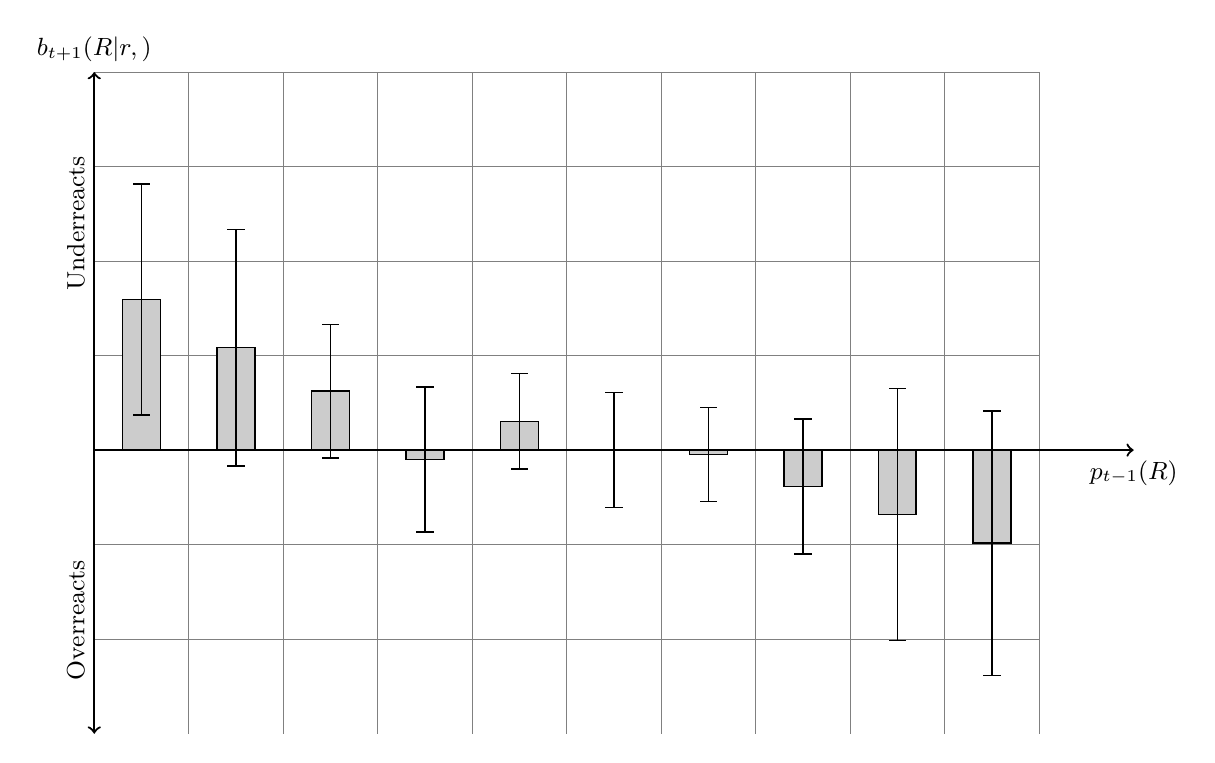
\begin{tikzpicture}[scale=12]
\draw[help lines,step=0.1] (0,-0.3) grid (1,0.4);
\filldraw[opaque,white!80!black] (0.03,0) rectangle (0.07,0.1592);
\draw[line width=0.6] (0.03,0) rectangle (0.07,0.1592);
\draw[line width=0.6,|-|] (0.05,0.0360) -- (0.05,0.2824);
\filldraw[opaque,white!80!black] (0.13,0) rectangle (0.17,0.1086);
\draw[line width=0.6] (0.13,0) rectangle (0.17,0.1086);
\draw[line width=0.6,|-|] (0.15,-0.0174) -- (0.15,0.2345);
\filldraw[opaque,white!80!black] (0.23,0) rectangle (0.27,0.0622);
\draw[line width=0.6] (0.23,0) rectangle (0.27,0.0622);
\draw[line width=0.6,|-|] (0.25,-0.0094) -- (0.25,0.1337);
\filldraw[opaque,white!80!black] (0.33,0) rectangle (0.37,-0.0100);
\draw[line width=0.6] (0.33,0) rectangle (0.37,-0.0100);
\draw[line width=0.6,|-|] (0.35,-0.0878) -- (0.35,0.0678);
\filldraw[opaque,white!80!black] (0.43,0) rectangle (0.47,0.0303);
\draw[line width=0.6] (0.43,0) rectangle (0.47,0.0303);
\draw[line width=0.6,|-|] (0.45,-0.0211) -- (0.45,0.0818);
\filldraw[opaque,white!80!black] (0.53,0) rectangle (0.57,0.0000);
\draw[line width=0.6] (0.53,0) rectangle (0.57,0.0000);
\draw[line width=0.6,|-|] (0.55,-0.0617) -- (0.55,0.0617);
\filldraw[opaque,white!80!black] (0.63,0) rectangle (0.67,-0.0046);
\draw[line width=0.6] (0.63,0) rectangle (0.67,-0.0046);
\draw[line width=0.6,|-|] (0.65,-0.0553) -- (0.65,0.0461);
\filldraw[opaque,white!80!black] (0.73,0) rectangle (0.77,-0.0387);
\draw[line width=0.6] (0.73,0) rectangle (0.77,-0.0387);
\draw[line width=0.6,|-|] (0.75,-0.1111) -- (0.75,0.0337);
\filldraw[opaque,white!80!black] (0.83,0) rectangle (0.87,-0.0682);
\draw[line width=0.6] (0.83,0) rectangle (0.87,-0.0682);
\draw[line width=0.6,|-|] (0.85,-0.2023) -- (0.85,0.0660);
\filldraw[opaque,white!80!black] (0.93,0) rectangle (0.97,-0.0986);
\draw[line width=0.6] (0.93,0) rectangle (0.97,-0.0986);
\draw[line width=0.6,|-|] (0.95,-0.2395) -- (0.95,0.0424);
\draw[line width=0.8,->]  (0,0) -- (1.1,0) node[below] {\small{$p_{t-1}(R)$}};
\draw[line width=0.8,<->] (0,-0.3) -- (0,0.4) node[above] {\small{$b_{t+1}(R|r,\xmark)$}};
\draw (0,0.24) node[above,rotate=90] {\small{Underreacts}};
\draw (0,-0.18) node[above,rotate=90] {\small{Overreacts}};
% ADD THEORY CURVE BELOW
\end{tikzpicture}
